\documentclass{article}
\usepackage{graphicx, color}


\setlength{\textwidth}{6.5in}
\setlength{\textheight}{8.0in}
\setlength{\oddsidemargin}{0in}
\setlength{\evensidemargin}{0in}
\setlength{\parskip}{2ex}
\setlength{\parindent}{0in}

%To display answers, replace "white" with "red" here;
\newcommand{\answer}[1]{\color{red}#1}

\begin{document}
\pagestyle{myheadings}\markright{
CU Boulder \hspace{0.5in} MATH 2510 - Introduction to Statistics }

\begin{center}
\textbf{\underbar{In-class Worksheet 11}}
\end{center}

This worksheet is an activity with the goal of simulating a sampling distribution of sample means. The first part of the activity is for each of you to generate a list of sample means. After the data is gathered, the second part directs you to use the results of the entire class to analyze the outcome.

\textbf{PART 1}

\begin{enumerate}

\item Attached to this page is a copy of a random number table for the population of digits \{0, 1, 2, 3, 4, 5, 6, 7, 8, 9\}. Assuming that this random distribution is uniform:

	\begin{enumerate}
	
	\item What is the population mean of the digits? 
	
	{\answer Since the frequency of all digits is equally weighed, $\mu = \frac{0+1+2+3+4+5+6+7+8+9}{10} = 4.5$.
	}
	
	\item What is the population standard deviation of the digits? 
	
	{\answer This could be done by hand (like the mean just was) or entering $L_1=\{0, 1, 2, 3, 4, 5, 6, 7, 8, 9\}$, \texttt{1-VarStats} indicates that $\sigma = 2.872281323$.
	} 
	\end{enumerate}
	
\item Repeat the following steps 10 times. In the end, you will have generated 10 different sample means. Please do NOT simply copy a classmate's values on this part, but please do your own work so that you really are generating your own list of sample means. 

	\begin{enumerate}
	
	\item {\em Randomly} select a spot on the random number table.
	
	\item Write down the next 10 digits listed from that spot horizontally (if you reach the end of a row, wrap around to the start of the next row to complete your list of 10). 
	
	\item Compute the mean of that sample of 10 random digits. 
	
	\end{enumerate}

\begin{center}	

\begin{tabular}{|c|c||c|}
\hline
Sample & List of 10 digits & Sample mean \\
\hline
1 & \hspace{3in} & \hspace{1in} \\
&&\\ \hline
2 & \hspace{3in} & \hspace{1in} \\
&&\\ \hline
3 & \hspace{3in} & \hspace{1in} \\
&&\\ \hline
4 & \hspace{3in} & \hspace{1in} \\
&&\\ \hline
5 & \hspace{3in} & \hspace{1in} \\
&&\\ \hline
6 & \hspace{3in} & \hspace{1in} \\
&&\\ \hline
7 & \hspace{3in} & \hspace{1in} \\
&&\\ \hline
8 & \hspace{3in} & \hspace{1in} \\
&&\\ \hline
9 & \hspace{3in} & \hspace{1in} \\
&&\\ \hline
10 & \hspace{3in} & \hspace{1in} \\
&&\\ \hline
\end{tabular}

\end{center}

\end{enumerate}

\textbf{PART 2}

\begin{enumerate}

\item Looking at the list of sample means, there should be a variety of values, but they are not uniformly distributed. What is the shape of the distribution for the sample means?

{\answer This will certainly vary from section to section, but the distributions should be roughly single-mound, symmetric.
} 

\item What is the mean of the sample means? 

{\answer Again, the specific answers will vary from section to section, but the outcome should be close to the population mean of $4.5$.
} 

\item What is the standard deviation of the sample means? 

{\answer Again, the specific answers will vary from section to section, but the outcome should not be too far from $\frac{2.872281323}{\sqrt{(10)}} \approx 0.9082951$.
} 

\item In Section 6.5, one of the most critical theorems in statistics is introduced; the Central Limit Theorem. Essentially it says that a sampling distribution for sample means (where the sample size for all samples is $n$) will have a distribution close to a normal distribution. Further, the mean of the sample means will equal the population mean $\mu$ and the standard deviation of the sample means will equal $\frac{\sigma}{\sqrt{(n)}}$. How did the simulation the class do match up to the theorem? 

	\begin{enumerate}
	
	\item Was the shape of the distribution of sample means approximately normal? 
	
	{\answer Answers will vary.
	} 
	
	\item Was the mean of the sample means close the the population mean $\mu$? 
	
	{\answer Answers will vary.
	} 
	
	\item What was the sample size for our sample means? 
	
	{\answer $n = 10$ 
	} 
	
	\item Was the standard deviation of the sample means close to the value $\frac{\sigma}{\sqrt{(n)}}$? 
	
	{\answer Answers will vary, but $\frac{\sigma}{\sqrt{(n)}} = \frac{2.872281323}{\sqrt{(10)}} \approx 0.9082951$.
	} 
	
	\end{enumerate}
	

\end{enumerate}

\vfill

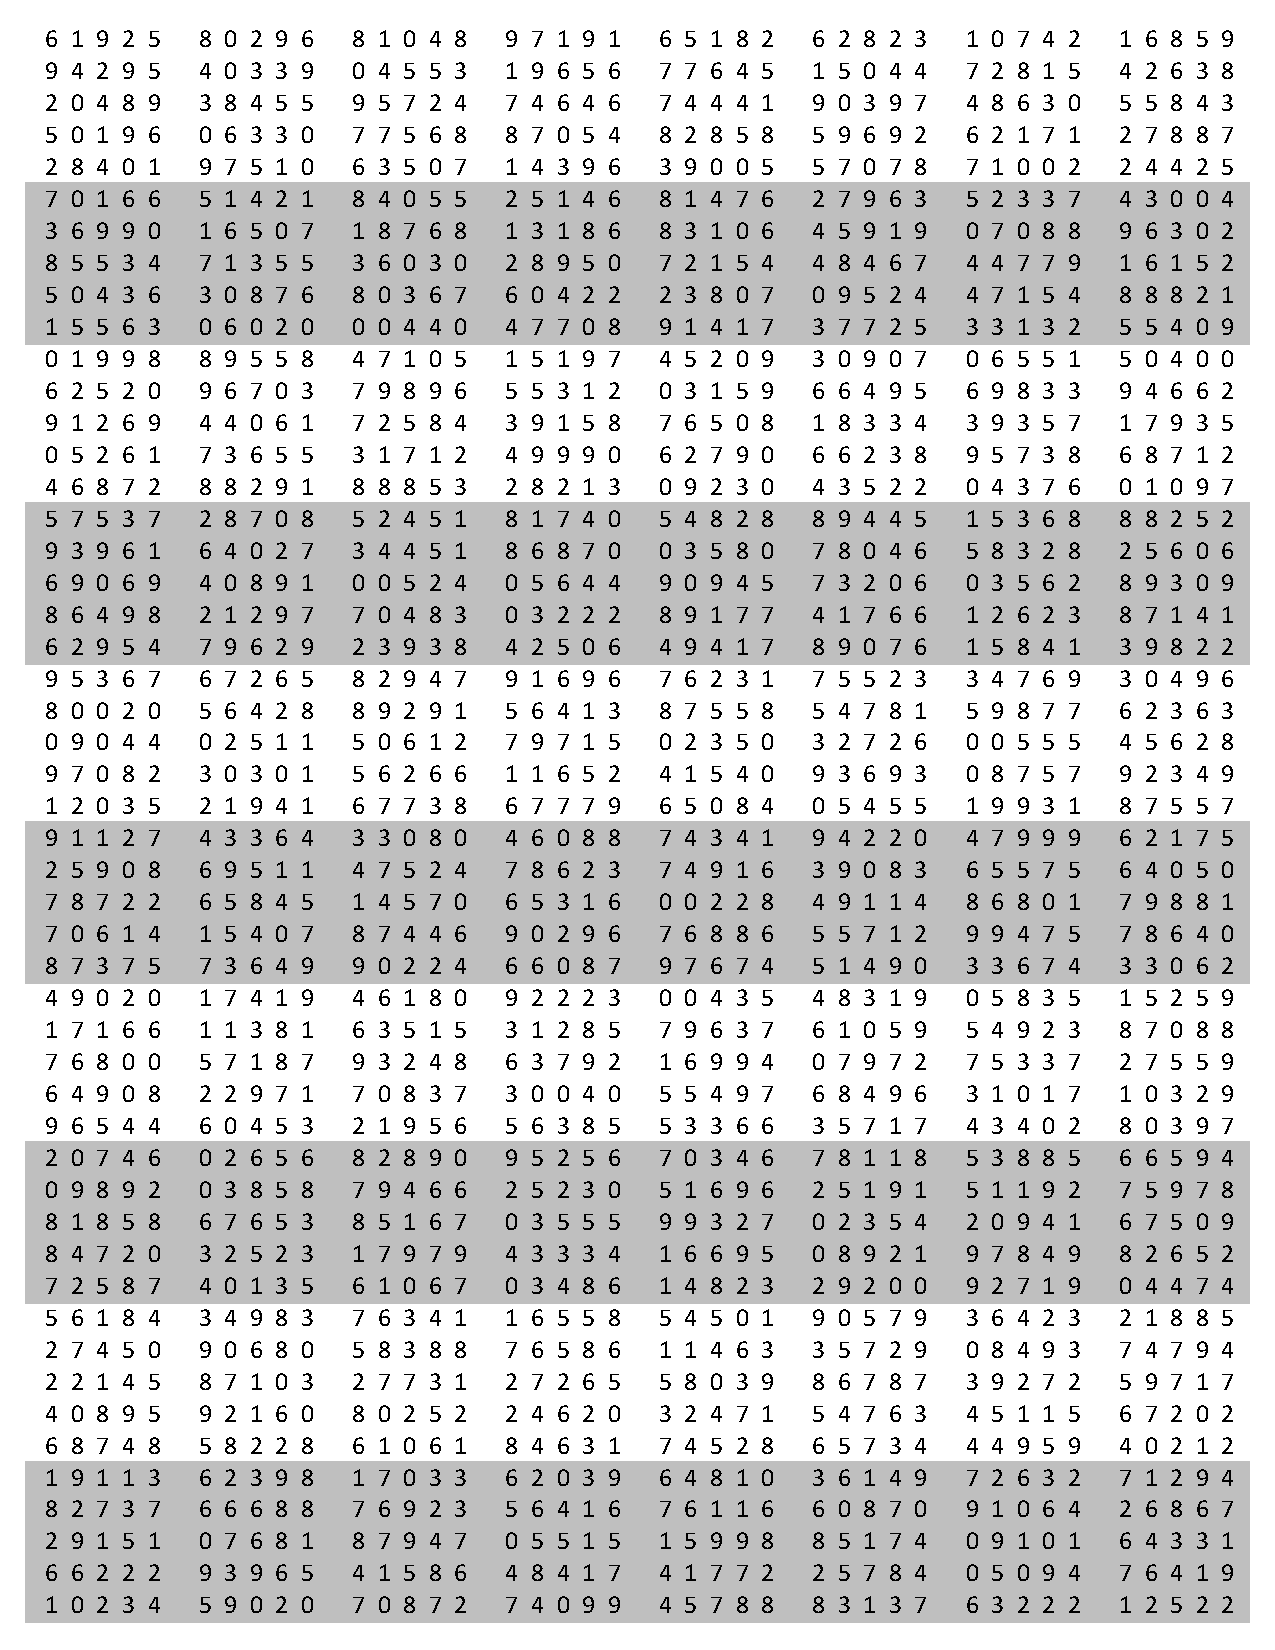
\includegraphics[scale=0.7]{RandNumbers.pdf}

\pagebreak

\begin{enumerate}

% Section 6.5 #8
\item Suppose a population has a distribution with $\mu = 72$ and $\sigma= 8$.
	\begin{enumerate}
	
	\item If we know nothing about the original population distribution and random samples of size $n=16$ are selected, why can't we say anything about the $\bar x$ distribution of sample means? 
	
	{\answer The sample size is too small to be certain what the resulting $\bar{x}$ distribution will look like.  In order to apply the Central Limit Theorem, which asserts that the $\bar{x}$ distribution is approximately normal, the sample size needs to be $n \geq 30$.
	} 

	\item If we know that the original population distribution is normal, then what can we say about the $\bar x$ distribution of random samples of $n=16$.  In this case, find $P(68 \leq \bar x \leq 73)$. 
	
	{\answer When the original population distribution is normal, then so will the $\bar{x}$ distribution, regardless of the size of the samples. 
	
	The $\bar{x}$ distribution still has a mean $\mu_{\bar{x}} = \mu = 72$, but the standard deviation is $\sigma_{\bar{x}} = \frac{\sigma}{\sqrt{n}} =\frac{8}{\sqrt{16}} = 2$. 
	
	$P(68 \leq \bar{x} \leq 73) = \texttt{normalcdf}(68, 73, 72, 2) \approx 0.6687124058$.
	} 
	
	\end{enumerate}
	
% Section 6.5 #14
\item The heights of 18-year-old men are approximately normally distributed, with a mean of 68 inches and a standard deviation of 3 inches.

	\begin{enumerate}
	
	\item What is the probability that an 18-year-old man selected at random is between 67 and 69 inches tall? 
	
	{\answer $P(67 < x < 69) = \texttt{normalcdf}(67, 69, 68, 3) \approx 0.2611171926$
	} 

	\item If a random sample of nine 18-year-old men are selected at random, what is the probability that the mean height of the sample $\bar x$ is between 67 and 69 inches? 
	
	{\answer  In this case, it is not the value of the random variable $x$ that we are considering, but rather the value of the mean $\bar{x}$ of samples of size $n = 9$.  
	
	Because the distribution of $x$ is normal, the distribution of $\bar{x}$ will be too.  Further, the mean of the $\bar{x}$ distribution is still 68, but the standard deviation of that distribution is $\frac{\sigma}{\sqrt{n}} = \frac{3}{\sqrt{9}} = 1$. 
	
	$P(67 < \bar{x} < 69) = \texttt{normalcdf}(67, 69, 68, 1) \approx 0.6826894809$
	} 

	\item Explain why the probability in part (b) is so much higher than the probability in part (a) even though they both refer to the same interval of heights (67 to 69 inches). 
	
	{\answer The standard deviation of the sample mean distribution is smaller than that of the original distribution, so there is less variance in the values.  That is, the mean height of a randomly selected sample of men is more likely to be close to the mean height of all men than a single randomly selected man's height is.
	} 
	%--
	\end{enumerate}

\pagebreak	
	
% Section 6.5 #16	
\item Let $x$ be a random variable that represents white blood cell count per cubic milliliter of whole blood.  Assume that $x$ has a distribution that is approximately normal with a mean of $\mu = 7500$ and estimated standard deviation of $\sigma = 1750$.  A test result of $x<3500$ is an indication of leukopenia.  This indicates bone marrow repression that may be the result of a viral infection.

	\begin{enumerate}
	
	\item What is the probability that, on a single test, $x$ is less than 3500? 
	
	{\answer $P(x<3500) = \texttt{normalcdf}(-1\mbox{E}99, 3500, 7500, 1750) \approx 0.01113549 \approx 1.11\%$
	} 

	\item Suppose a doctor uses the average $\bar x$ for two tests taken about a week apart.  What can we say about the probability distribution of $\bar x$?  What is the probability that $\bar x < 3500$? 
	
	{\answer Because $x$ has a distribution that is approximately normal, the distribution of the averages of the samples (even with size as small as $n=2$) is also normal.  The mean of the distribution of averages is still $7500$, however, the standard deviation is reduced to $\frac{\sigma}{\sqrt{n}} = \frac{1750}{\sqrt{2}}.$ 
	
	$P(\bar{x} < 3500) = \texttt{normalcdf}(-1\mbox{E}99, 3500, 7500, 1750/\sqrt(2)) = 0.0006135861 \approx 0.061\%$
	} 

	\item Repeat part (b) but with $n=3$ tests. 
	
	{\answer Again, the distribution of the averages of three test results is normal, with mean $7500$ and standard deviation $\frac{\sigma}{\sqrt{n}} = \frac{1750}{\sqrt{3}}$. 
	
	$P(\bar{x} < 3500) = \texttt{normalcdf}(-1\mbox{E}99, 3500, 7500, 1750\sqrt(3)) = 0.00003763633 \approx 0.0038\%$
	} 

	\item How did the probabilities change as $n$ increased?  What do such results imply about a patient that has $\bar x < 3500$ for 3 those tests?  
	
	{\answer Although it is possible for an isolated random test to indicate a low count when absolutely nothing is wrong, the greater $n$ is, it becomes less and less likely that the average of the tests will be less than 3500 when absolutely nothing is wrong. 
	
	According to part (c), the likelihood that the average of 3 tests is less than 3500 just by random chance is only $0.00003763633$.  So, for a patient with such results, the probability is extremely high that they do, in fact, have leukopenia.
	} 
	%--
	\end{enumerate}
	
%Chapter 6 Review #23-ish
\item Assume that IQ scores are normally distributed, with a standard deviation of 15 points and a mean of 100 points.  If 10 people are chosen at random, what is the probability that the sample mean of their IQ scores will not differ from the population mean by more than 2 points? 

{\answer In this case, we are looking for the probability that the sample mean $\bar{x}$ falls between 98 and 102 points.  Because the distribution of IQ scores is normal, the Central Limit Theorem can be applied with $\mu_{\bar{x}} = 100$ and $\sigma_{\bar{x}} =\frac{15}{\sqrt{10}}$. 

So, $P(98 \leq \bar{x} \leq 102) = \texttt{normalcdf}(98, 102, 100, \frac{15}{\sqrt{10}}) \approx 0.3267099507 \approx 32.67\%$.
} 

%Chapter 6 Review #24
\item A large tank of fish from a hatchery is being delivered to a lake.  The hatchery claims that the mean length of fish in the tank is 15 inches, and the standard deviation is 2 inches.  A random sample of 36 fish is taken from the tank.  Let $\bar{x}$ be the mean length of the sample.  What is the probability that $\bar{x}$ is within $0.5$ inches of the claimed population mean? 

{\answer Although there is no indication that the distribution of lengths of the fish is normal, the sample size is greater than 30, so the Central Limit Theorem applies.  So, we can apply the \texttt{normalcdf} function with $\mu_{\bar{x}}=15$ and $\sigma_{\bar{x}} = 2/\sqrt{36} = 1/3$. 

$\texttt{normalcdf(14.5, 15.5, 15, 1/3)} \approx 0.8663855426 \approx 86.64\%$
} 

\end{enumerate}

\end{document}

